% ============================ Part 7: RLVR & GRPO ============================
\section{Part 7 $\cdot$ RLVR \& GRPO}
\partslide{7}{Verifiable rewards \& GRPO}{learning to reason}

\begin{frame}{Reasoning models: think first, answer later}
\begin{columns}[T]
\begin{column}{0.52\textwidth}
\centering
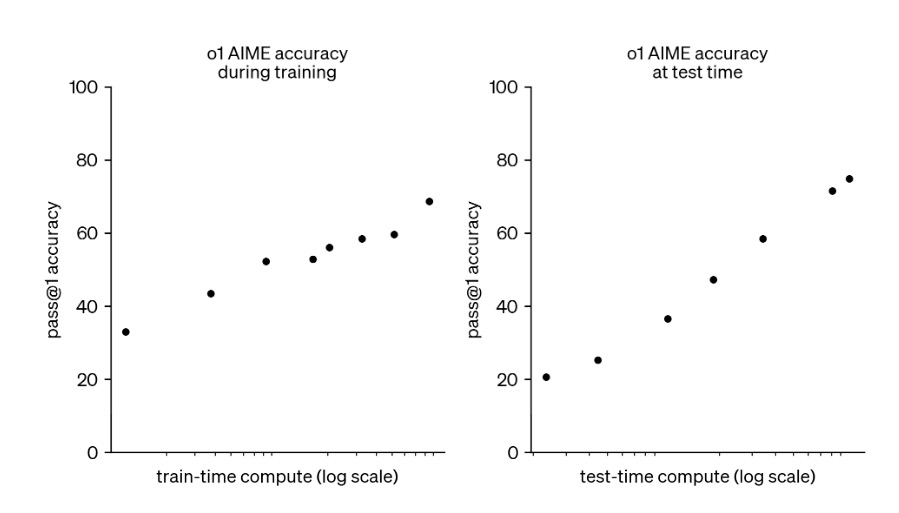
\includegraphics[width=\textwidth]{figs/o1_aime.png}\\[2pt]
\scriptsize OpenAI o1 (2024): AIME accuracy grows with RL training compute (left) \emph{and} with thinking time at test time (right).
\end{column}
\begin{column}{0.46\textwidth}
\begin{itemize}\setlength{\itemsep}{6pt}
  \item A \textbf{reasoning model} writes a long chain of thought \emph{before} its final answer --- CoT (Part 3) as a learned default.
  \item \textbf{o1} (Sept.\ 2024): closed recipe, clear message --- RL training + ``thinking time''.
  \item \textbf{DeepSeek-R1} (Jan.\ 2025): open weights, open recipe --- the algorithm is \textbf{GRPO}.
\end{itemize}
\end{column}
\end{columns}
\vspace{6pt}
\keybox{Nobody writes the chains of thought. Where does the training signal come from? From checking the \emph{final answer}.}
\end{frame}

\begin{frame}{Verifiable rewards: let a program be the judge}
\begin{columns}[T]
\begin{column}{0.5\textwidth}
\textbf{RL with verifiable rewards (RLVR):}
\[
  R(x,y) = \begin{cases}1 & \text{answer in } y \text{ passes the checker}\\ 0 & \text{otherwise}\end{cases}
\]
\begin{itemize}\setlength{\itemsep}{5pt}
  \item \textbf{Math:} compare the boxed final answer with the answer key.
  \item \textbf{Code:} run the unit tests.
  \item \textbf{Logic, games, formal proofs:} a checker exists.
  \item Plus a small \textbf{format reward} (answer in \texttt{\textbackslash boxed\{\}}) so the output can be parsed.
\end{itemize}
\end{column}
\begin{column}{0.48\textwidth}
\centering
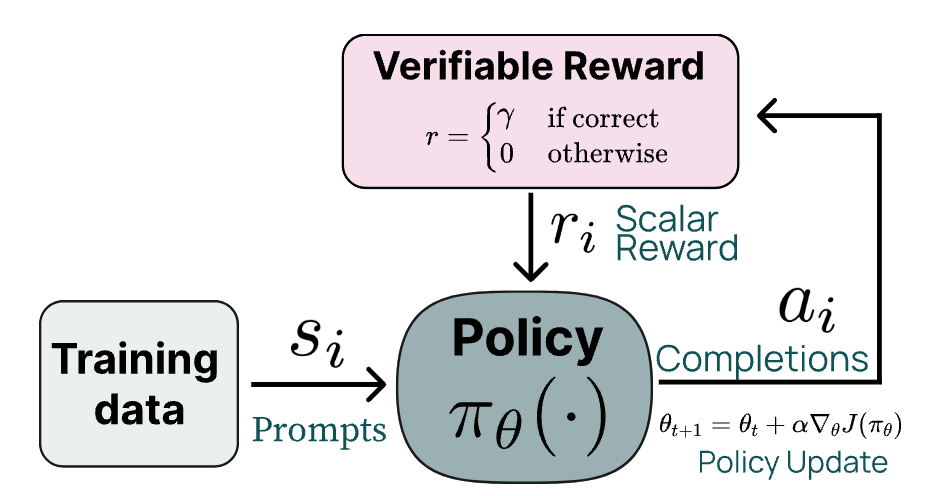
\includegraphics[width=0.95\textwidth]{figs/rlvr_diagram.png}\\[2pt]
\scriptsize The RLVR loop (T\"ulu 3, 2024): prompts in, completions out, a verifier scores them, policy gradient updates $\theta$.
\end{column}
\end{columns}
\vspace{4pt}
\keybox{No human label per sample, no learned reward model to fool, unlimited re-checking.}
\end{frame}

\begin{frame}{Why RL, not just SFT on worked solutions?}
\centering
\renewcommand{\arraystretch}{1.4}\setlength{\tabcolsep}{4pt}
\begin{tabular}{@{}p{2.4cm}p{5.3cm}p{5.6cm}@{}}
\toprule
 & \textbf{SFT on human solutions} & \textbf{RLVR}\\
\midrule
data & a person must write every full solution & only the \emph{answer key} is needed\\
what is optimized & imitate the human's steps (maybe clumsy) & the \emph{outcome}; the model finds its own path\\
distribution & learns from human-written text & learns from \emph{its own} samples --- what it faces at inference\\
behaviors & only what was demonstrated & can \emph{discover} re-checking, backtracking, trying another approach\\
\bottomrule
\end{tabular}
\vspace{10pt}

\keybox{RLHF (Part 6) makes models \emph{sound} aligned --- polite, helpful, safe --- but does not make them reason better. For reasoning the reward must be about \emph{correctness}.}
\end{frame}

\begin{frame}{From PPO to GRPO: drop the critic, use the group}
\begin{columns}[T]
\begin{column}{0.44\textwidth}
\begin{itemize}\setlength{\itemsep}{6pt}
  \item PPO's baseline $b(x)$ comes from a learned \textbf{value network} --- a second LLM-sized model trained alongside the policy.
  \item Expensive: doubles memory and compute.
  \item Fragile: with one reward at the \emph{end} of a long chain, token-level value estimates are noisy.
\end{itemize}
\keybox{\textbf{GRPO} (DeepSeekMath, 2024): we already sample several responses per question --- let them be \emph{each other's baseline}. No critic.}
\end{column}
\begin{column}{0.54\textwidth}
\centering
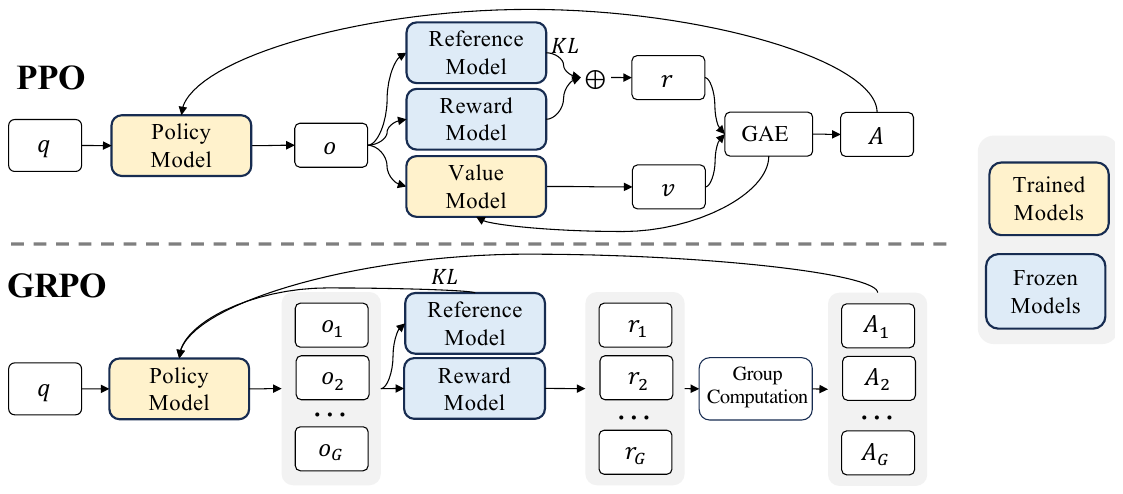
\includegraphics[width=\textwidth]{figs/ppo_vs_grpo.png}\\[2pt]
\scriptsize PPO keeps a value model (yellow = trained); GRPO replaces it by a ``group computation'' over $G$ sampled outputs.
\end{column}
\end{columns}
\end{frame}

\begin{frame}{GRPO at a glance}
\begin{center}
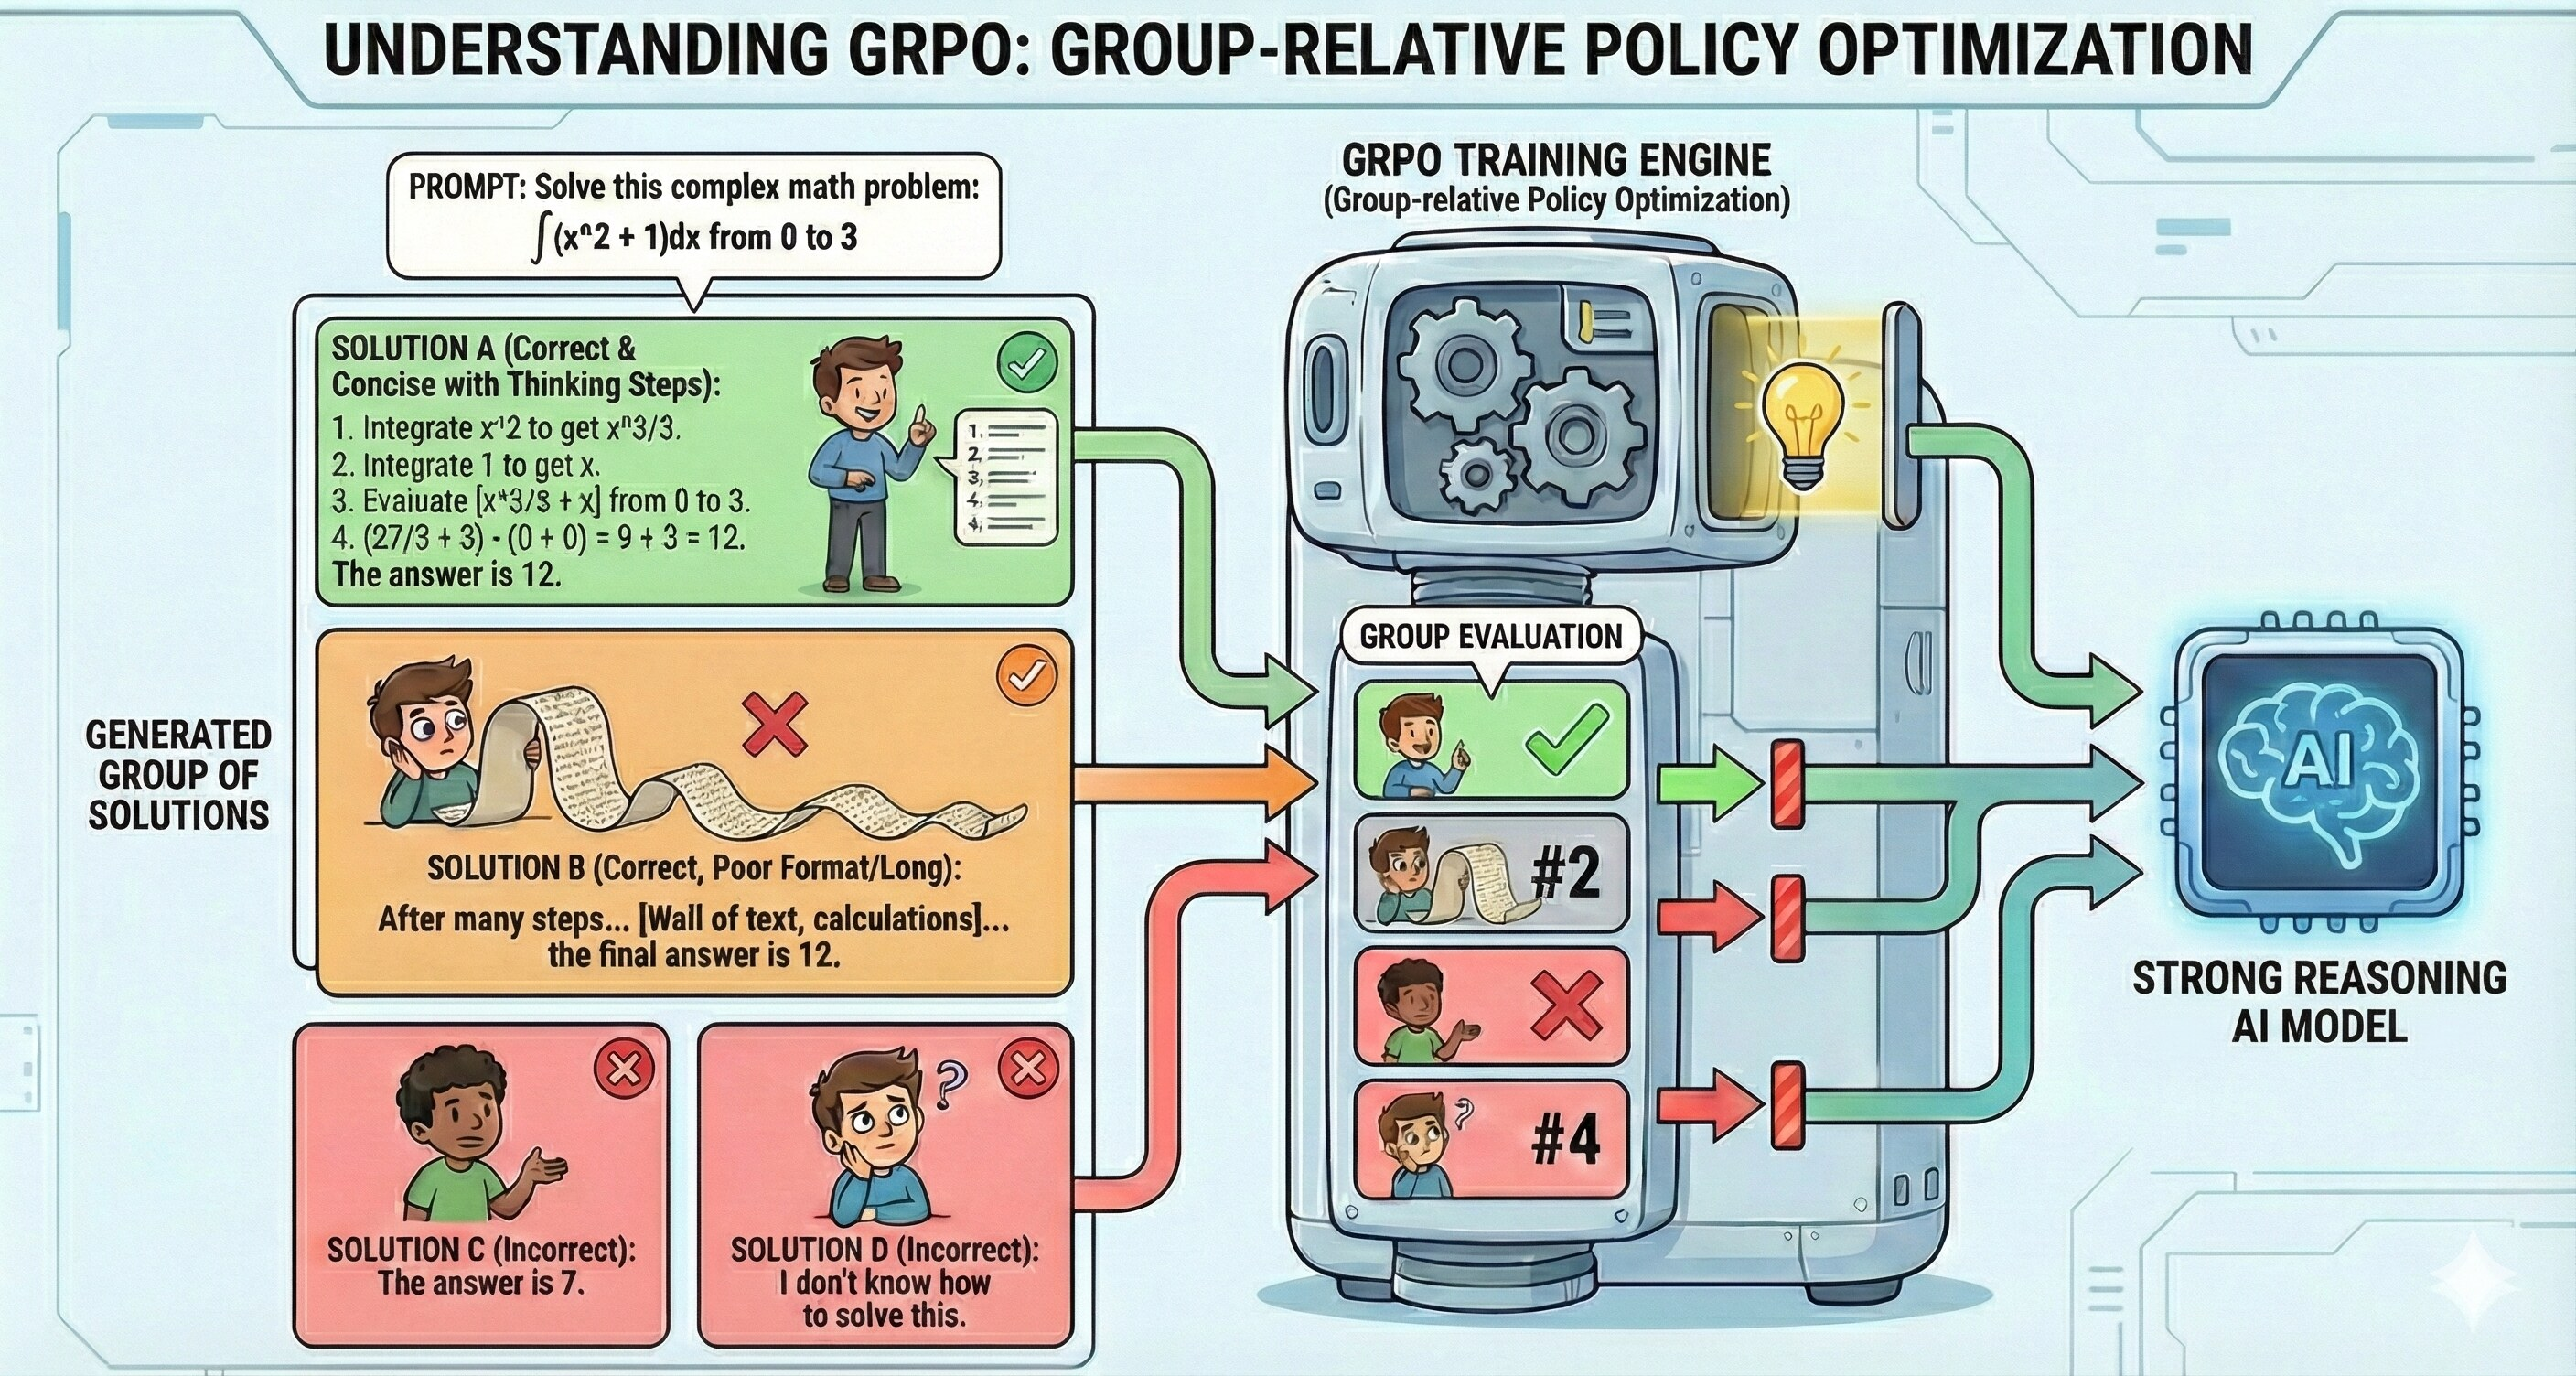
\includegraphics[width=0.8\textwidth]{figs/grpo_illustration.jpg}
\end{center}
\vspace{-2pt}
\centering Sample a \textbf{group} of solutions to one problem $\to$ check each one $\to$ reinforce the ones that did better than the group.
\end{frame}

\begin{frame}{GRPO step 1: sample a group of answers to the same question}
\begin{center}
\begin{tikzpicture}[font=\scriptsize,>=Latex]
  \node[draw,rounded corners,fill=softgray,minimum width=2.4cm,minimum height=0.9cm,align=center] (q) at (0,0) {\textbf{question $q$}\\``Find all $a$ such that \dots''};
  \node[draw,rounded corners,fill=uvanavy!12,minimum width=2.1cm,minimum height=0.9cm,align=center] (pi) at (3.0,0) {\textbf{policy $\pi_{\text{old}}$}\\sample with $\tau>0$};
  \draw[->,thick] (q) -- (pi);
  \foreach \i/\y/\r/\c in {1/1.75/1/okgreen,2/1.25/0/badred,3/0.75/1/okgreen,4/0.25/0/badred,5/-0.25/0/badred,6/-0.75/0/badred,7/-1.25/1/okgreen,8/-1.75/0/badred}{
    \node[draw,rounded corners,fill=white,minimum width=2.3cm,minimum height=0.38cm,font=\tiny] (o\i) at (6.1,\y) {response $o_{\i}$ \; (reasoning \dots\ answer)};
    \draw[->] (pi.east) -- (o\i.west);
    \node[draw,rounded corners,fill=\c!15,draw=\c!70!black,minimum width=0.75cm,minimum height=0.34cm,font=\tiny] (r\i) at (8.8,\y) {$r_{\i}=\r$};
    \draw[->] (o\i) -- (r\i);
  }
  \node[draw,rounded corners,fill=uvaorange!15,draw=uvaorange!80!black,minimum width=1.3cm,minimum height=0.8cm,align=center] (v) at (10.7,0.9) {\textbf{verifier}\\answer key};
  \draw[->,dashed,uvaorange!80!black] (v.west) -- (r3.east);
  \node[font=\scriptsize,align=center] at (10.7,-0.9) {$G = 8$ samples\\3 correct, 5 wrong};
\end{tikzpicture}
\end{center}
\begin{itemize}\setlength{\itemsep}{4pt}
  \item For each question $q$: sample $G$ responses from $\pi_{\text{old}}(\cdot\mid q)$ with temperature (Part 2); the verifier scores each, $r_i\in\{0,1\}$.
  \item Typical: $G = 8$--$64$ per question, hundreds of questions per batch. The model's \emph{own attempts} are the data.
\end{itemize}
\end{frame}

\begin{frame}{GRPO step 2: the advantage is relative to the group}
\[
  \hat{A}_i = \frac{r_i - \operatorname{mean}(r_1,\dots,r_G)}{\operatorname{std}(r_1,\dots,r_G) + \varepsilon}
  \qquad\text{and the same } \hat A_i \text{ goes to \emph{every token} of response } o_i.
\]
\vspace{4pt}
\begin{itemize}\setlength{\itemsep}{8pt}
  \item The \textbf{baseline is the group mean} --- ``how hard is this question for the current model'' --- obtained for free.
  \item Dividing by the std puts easy and hard questions on one scale.
  \item All right or all wrong $\Rightarrow$ $\hat A_i = 0$: no gradient. Learning happens where the model \emph{sometimes} succeeds.
\end{itemize}
\vspace{6pt}
\callback{Part 5}{advantage = reward $-$ baseline; the baseline now comes from samples instead of a critic.}
\end{frame}

\begin{frame}{GRPO step 2: a worked example}
\newcommand{\yw}{y_w}
Rewards of the $G=8$ samples from step 1: \; $1,\,0,\,1,\,0,\,0,\,0,\,1,\,0$
\begin{align*}
  \operatorname{mean} &= 3/8 = 0.375, \qquad \operatorname{std} = \sqrt{0.375\cdot 0.625} \approx 0.48\\[4pt]
  \hat A_{\text{correct}} &= \frac{1 - 0.375}{0.48} \approx \green{+1.29}, \qquad\qquad
  \hat A_{\text{wrong}} = \frac{0 - 0.375}{0.48} \approx \red{-0.77}
\end{align*}
\vspace{2pt}
\begin{itemize}\setlength{\itemsep}{8pt}
  \item The 3 correct responses are pushed \emph{up} with weight $+1.29$; the 5 wrong ones pushed \emph{down} with $-0.77$.
  \item Had 7 of 8 been correct: $+0.38$ for the correct ones and $-2.65$ for the lone mistake --- the rare failure is what gets corrected.
  \item Had 0 of 8 been correct: all advantages $0$ --- this question teaches nothing \emph{yet}.
\end{itemize}
\end{frame}

\begin{frame}{GRPO step 3: the objective}
\[
  J_{\text{GRPO}}(\theta) = \E_{q,\{o_i\}}\Bigg[\frac{1}{G}\sum_{i=1}^{G}\frac{1}{|o_i|}\sum_{t=1}^{|o_i|}
  \underbrace{\min\!\Big(\rho_{i,t}\,\textcolor{uvaorange!85!black}{\hat A_i},\;\operatorname{clip}(\rho_{i,t},1-\epsilon,1+\epsilon)\,\textcolor{uvaorange!85!black}{\hat A_i}\Big)}_{\textcolor{okgreen!70!black}{\text{PPO clipping (Part 5)}}}\Bigg]
  -\underbrace{\beta\,\mathrm{KL}(\pi_\theta\,\|\,\pi_{\text{ref}})}_{\textcolor{okgreen!70!black}{\text{KL leash}}}
\]
\centering\small $\rho_{i,t} = \pi_\theta(o_{i,t}\mid q, o_{i,<t}) \,/\, \pi_{\text{old}}(o_{i,t}\mid q, o_{i,<t})$ is the per-token probability ratio; $\hat A_i$ comes from step 2.
\vspace{8pt}

\raggedright
\textbf{How to read it.} Ignore the clip and KL for a moment ($\rho\approx 1$): the gradient is
\[
  \frac{1}{G}\sum_i \hat A_i \cdot \nabla_\theta \log\pi_\theta(o_i\mid q)\quad\text{(per token)}
\]
\keybox{= the \textbf{SFT gradient on the model's own responses, weighted by advantage}: correct chains reinforced, wrong ones suppressed; clip and KL keep each step small.}
\end{frame}

\begin{frame}{GRPO step 3: the algorithm}
\begin{columns}[T]
\begin{column}{0.5\textwidth}
\textbf{In five lines:}
\begin{enumerate}\setlength{\itemsep}{5pt}
  \item Take a batch of questions; set $\pi_{\text{old}}\leftarrow\pi_\theta$.
  \item Sample $G$ responses per question from $\pi_{\text{old}}$.
  \item Score with the verifier; compute $\hat A_i$ per group.
  \item A few gradient steps on $J_{\text{GRPO}}$ (clipped, KL-regularized).
  \item Repeat for thousands of batches.
\end{enumerate}
\vspace{4pt}
\keybox{No reward model, no value model: the policy, a frozen reference copy, and a checker.}
\end{column}
\begin{column}{0.48\textwidth}
\centering
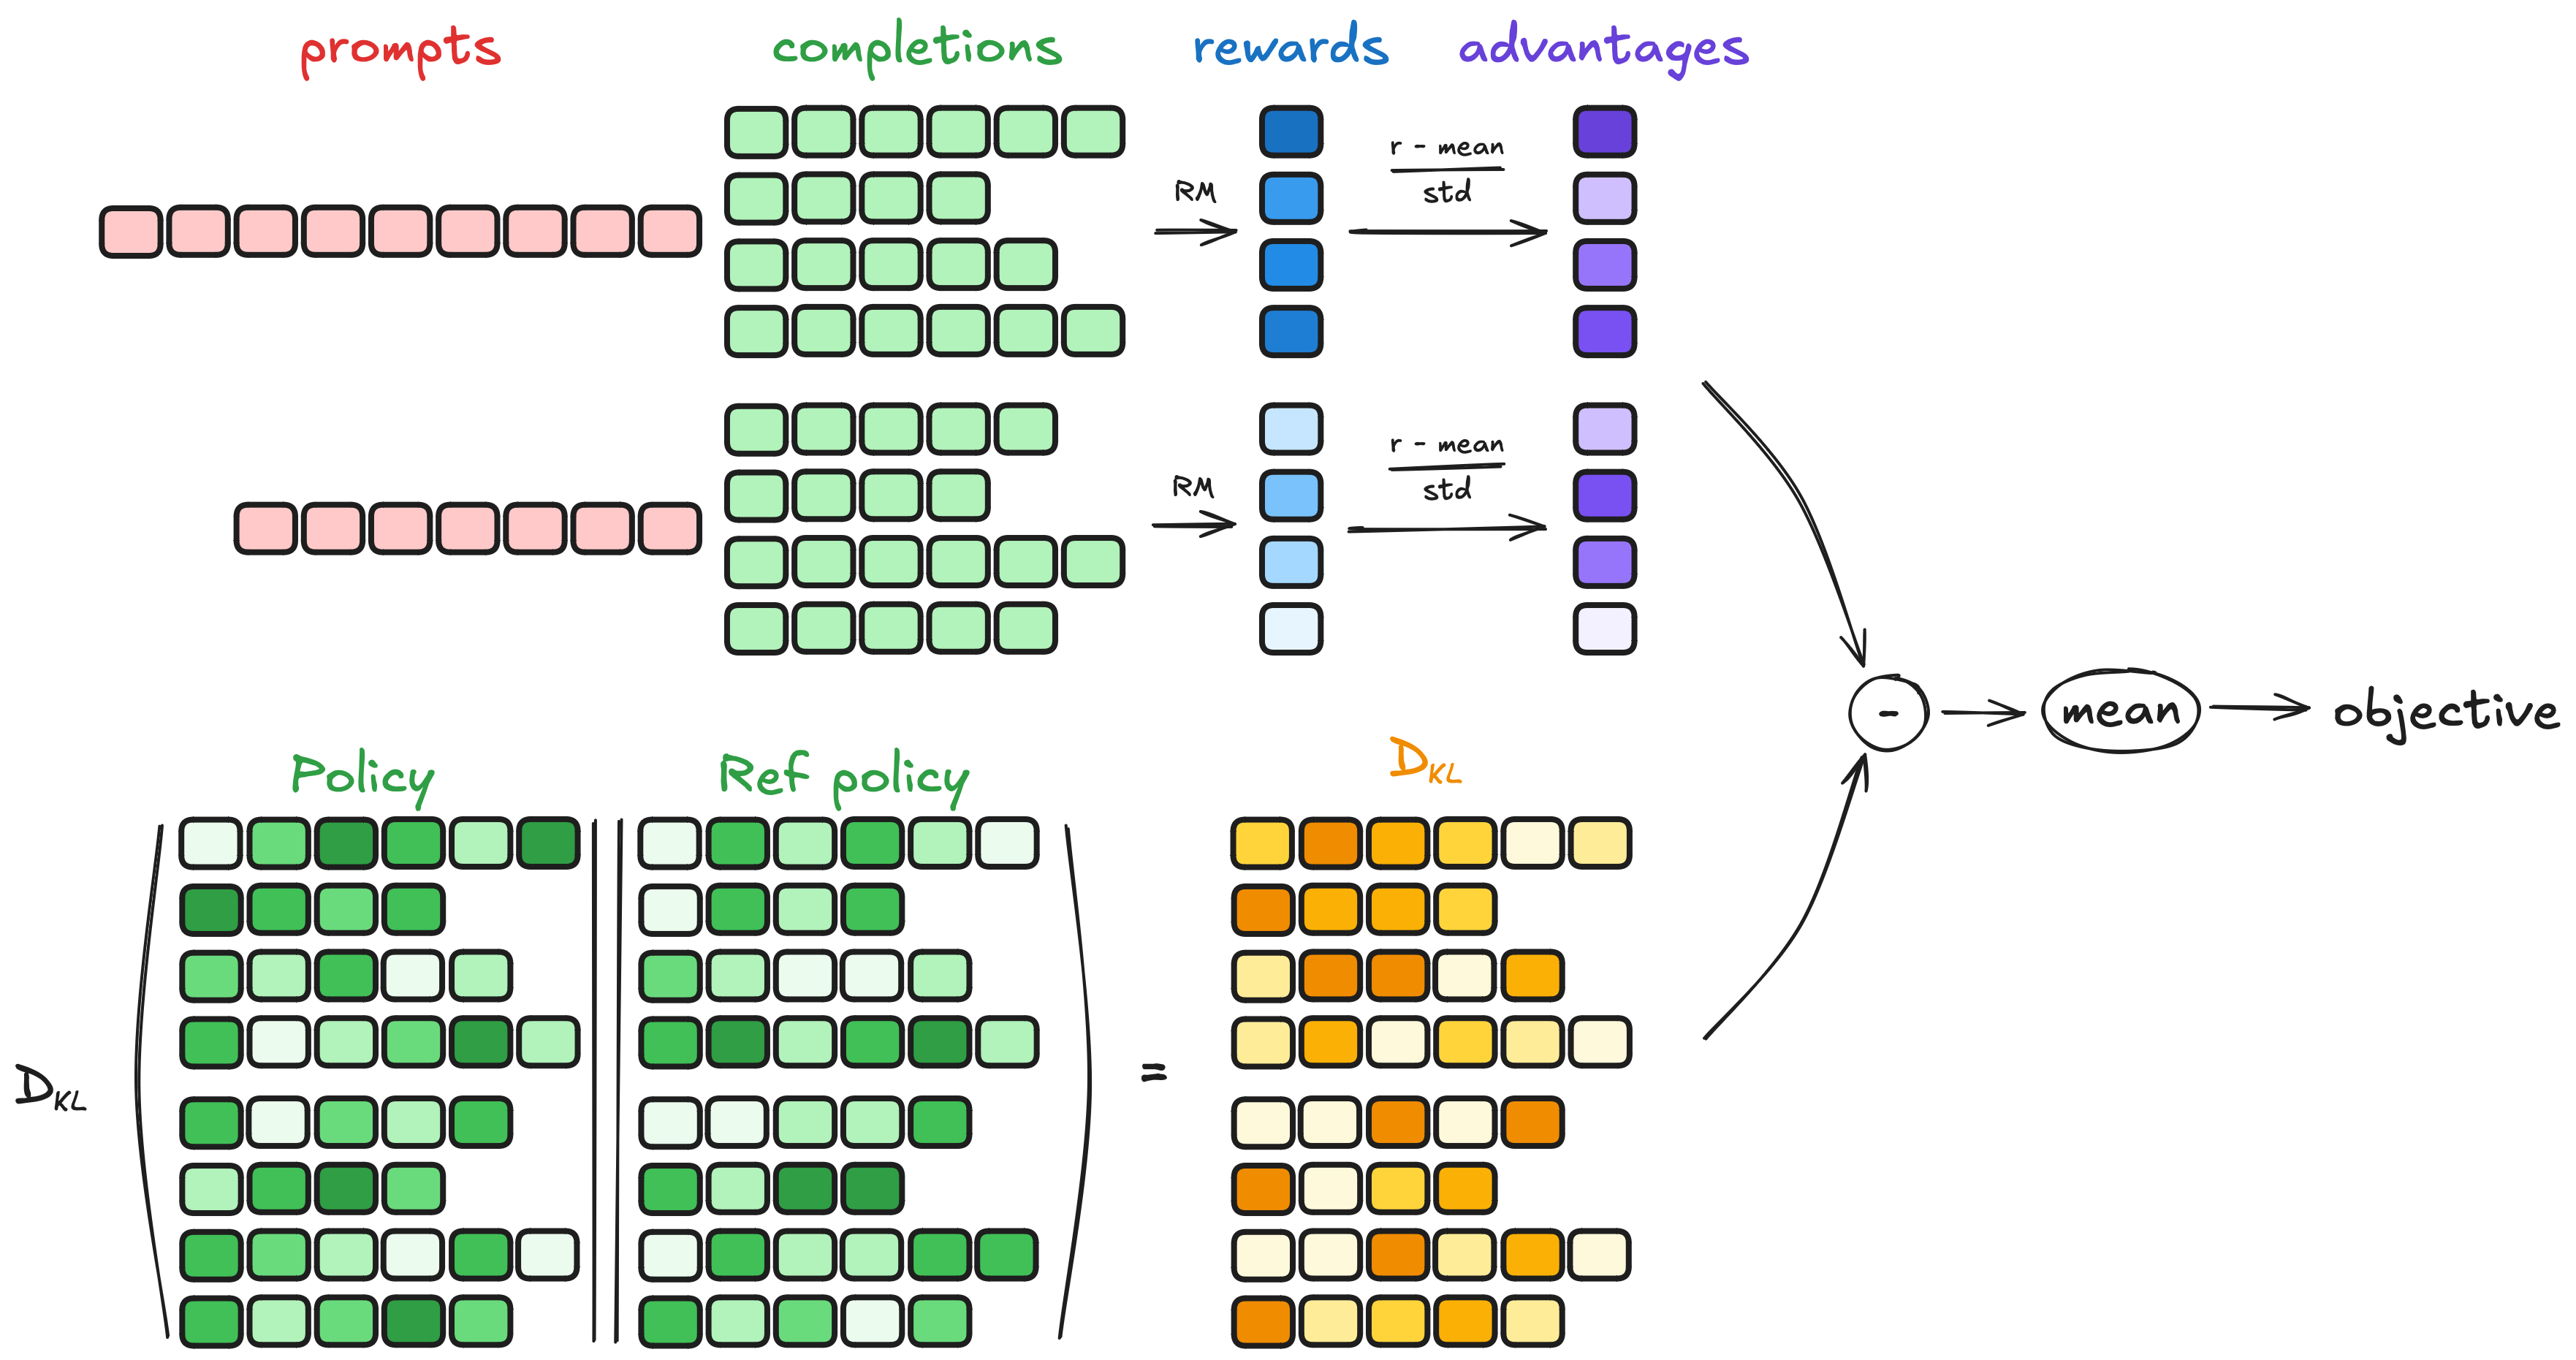
\includegraphics[width=\textwidth]{figs/trl_grpo_visual.png}\\[2pt]
\scriptsize What a GRPO trainer computes (Hugging Face TRL): completions $\to$ rewards $\to$ group-normalized advantages; policy vs.\ reference log-probs $\to$ KL; both $\to$ the objective.
\end{column}
\end{columns}
\end{frame}

\begin{frame}{What happens during training: DeepSeek-R1-Zero}
\begin{columns}[T]
\begin{column}{0.5\textwidth}
\centering
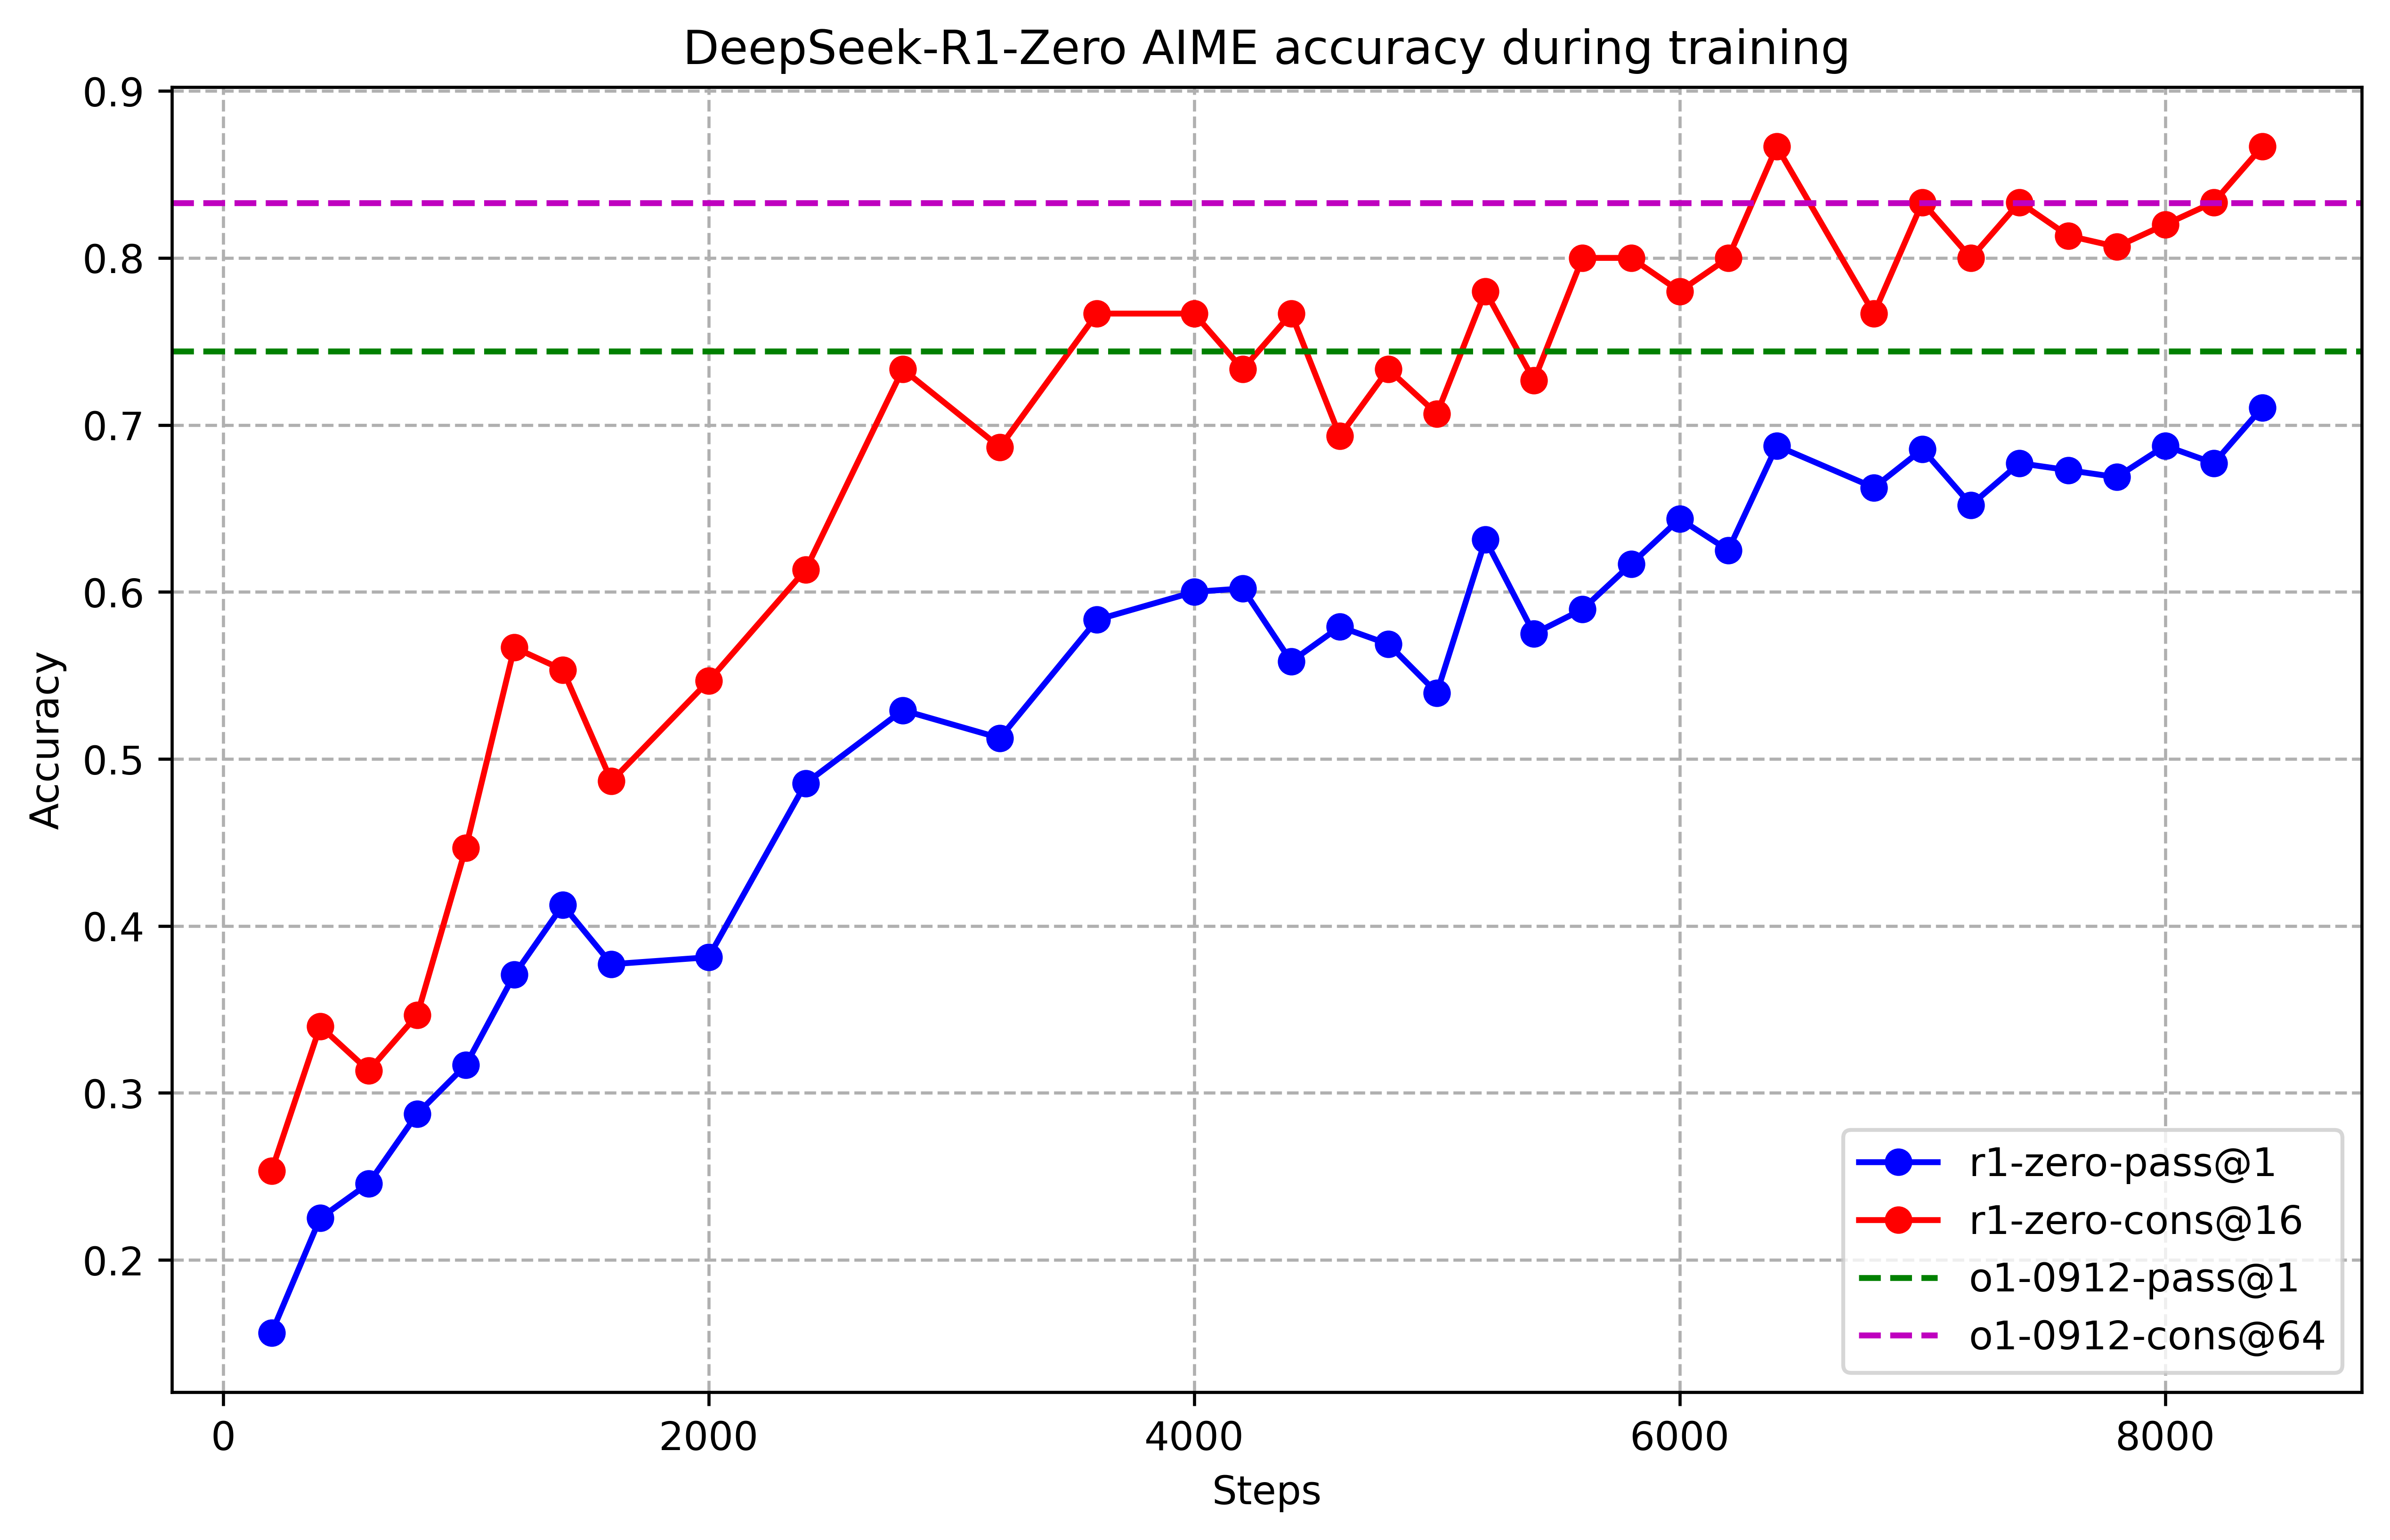
\includegraphics[width=0.85\textwidth]{figs/r1zero_aime_curve.png}\\[1pt]
\scriptsize AIME 2024 accuracy during GRPO training (pure RL from the base model, no SFT).
\end{column}
\begin{column}{0.48\textwidth}
\centering
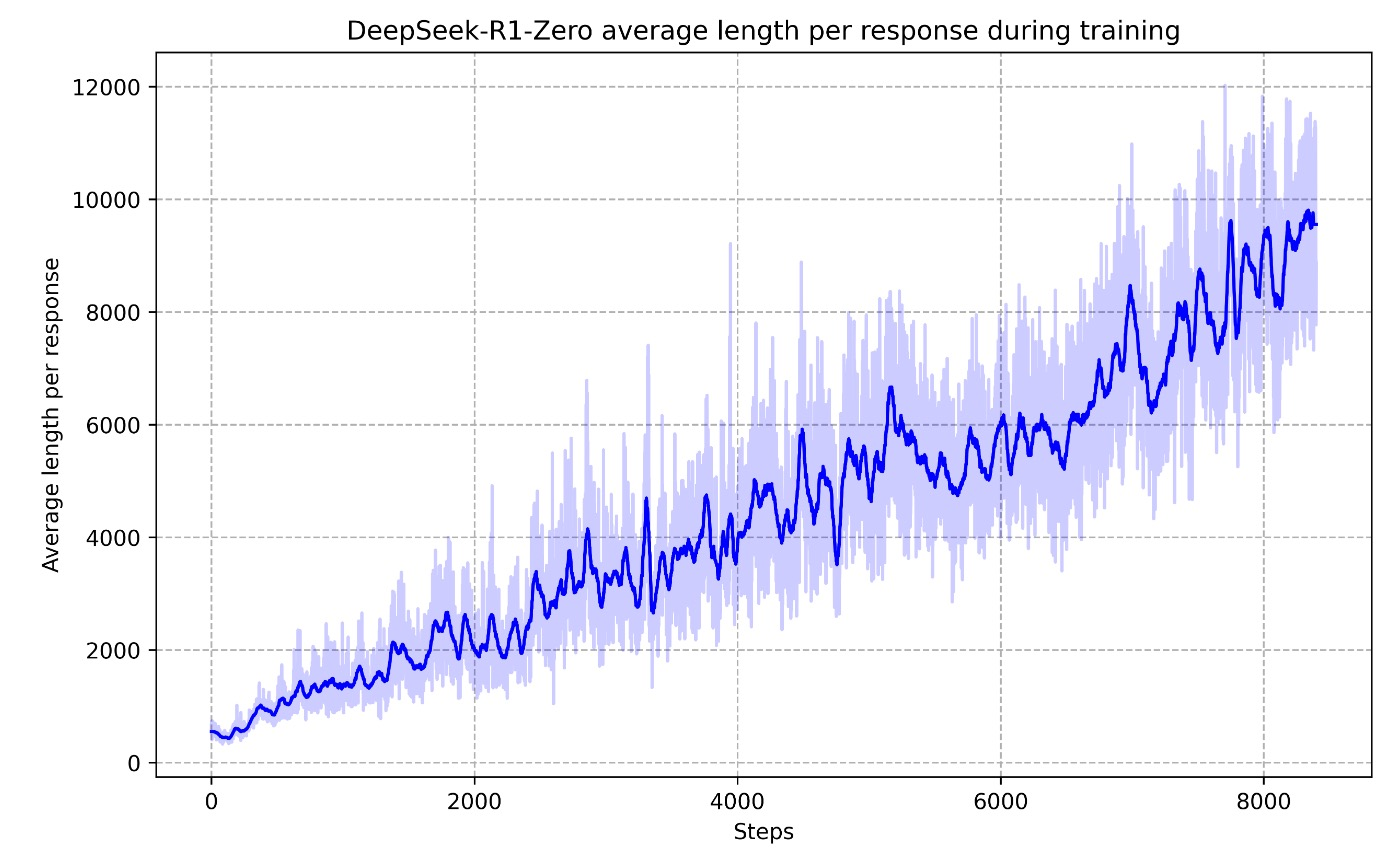
\includegraphics[width=0.85\textwidth]{figs/r1_length.png}\\[1pt]
\scriptsize Average response length during training: the model \emph{learns to think longer}.
\end{column}
\end{columns}
\vspace{6pt}
\begin{itemize}\setlength{\itemsep}{4pt}
  \item AIME pass@1: \textbf{15.6\% $\to$ 71.0\%} (86.7\% with majority vote over 64 samples) --- on par with o1.
  \item The reward only says \emph{correct / incorrect}; longer thinking, re-checking, and backtracking \textbf{emerged} because they raise the chance of a correct answer.
\end{itemize}
\end{frame}

\begin{frame}{The ``aha moment''}
\begin{columns}[T]
\begin{column}{0.6\textwidth}
\centering
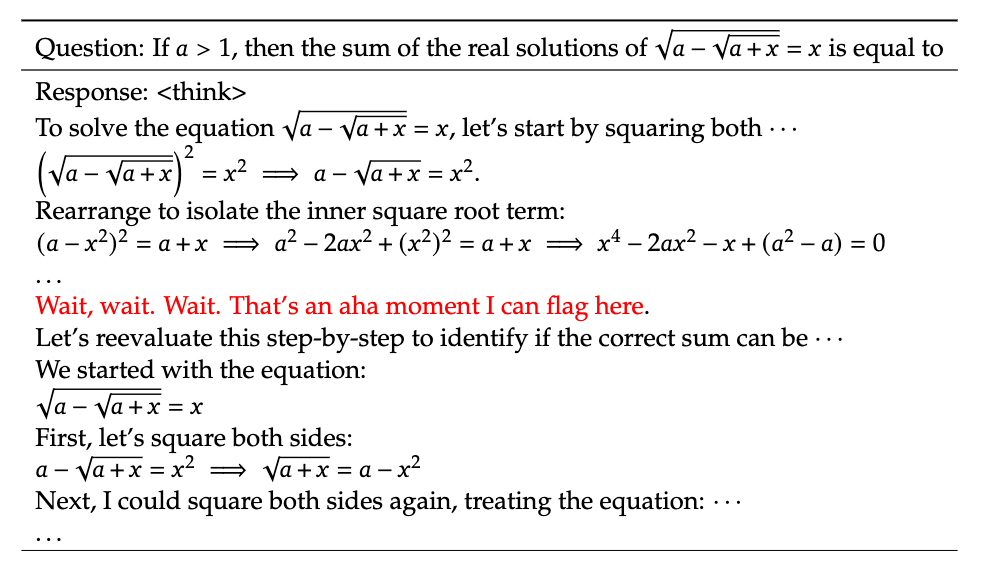
\includegraphics[width=\textwidth]{figs/r1_aha.png}\\[2pt]
\scriptsize An intermediate R1-Zero checkpoint, mid-solution (DeepSeek-AI, 2025).
\end{column}
\begin{column}{0.38\textwidth}
\begin{itemize}\setlength{\itemsep}{7pt}
  \item The model stops, flags a problem with its own approach, and \emph{re-evaluates} --- in a tone nobody put in the training data.
  \item This is what ``learning from evaluation'' buys: behaviors that \emph{work} get reinforced, whether or not a human would have written them.
  \item RL optimizes \emph{the reward} --- not readability or brevity; hence R1 adds SFT and RLHF stages after R1-Zero.
\end{itemize}
\end{column}
\end{columns}
\end{frame}

\begin{frame}{Open questions (active research --- including at UVA)}
\begin{columns}[T]
\begin{column}{0.52\textwidth}
\centering
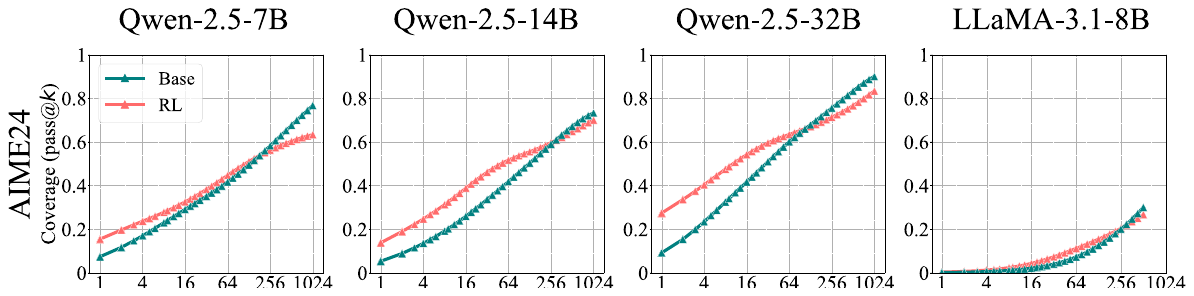
\includegraphics[width=\textwidth]{figs/passk.png}\\[2pt]
\scriptsize pass@$k$ (solved if \emph{any} of $k$ samples is correct) vs.\ $k$ on AIME24: the RL model wins at small $k$, the \emph{base} model catches up at large $k$ (Yue et al., 2025).
\end{column}
\begin{column}{0.46\textwidth}
\begin{itemize}\setlength{\itemsep}{6pt}
  \item \textbf{New reasoning, or sharper sampling?} Much of RLVR's gain is sampling efficiency; RL can also narrow the paths the model explores (``diversity collapse'').
  \item \textbf{Exploration and diversity} of reasoning trajectories: entropy bonuses, asymmetric clipping and dynamic sampling (DAPO), prolonged RL with KL resets (ProRL).
  \item \textbf{Sparse, outcome-only rewards} vs.\ step-level rewards; reward hacking even with verifiers.
\end{itemize}
\end{column}
\end{columns}
\end{frame}

\begin{frame}{Hands-on: two Colab notebooks}
\begin{columns}[T]
\begin{column}{0.53\textwidth}
\textbf{Notebook 1 --- preference fine-tuning (DPO)}
\begin{itemize}\setlength{\itemsep}{2pt}
  \item SFT model (Zephyr-7B, QLoRA) + UltraFeedback preference pairs.
  \item Watch accuracy, margin, and the implicit rewards (Part 6 curves).
\end{itemize}
\vspace{4pt}
\textbf{Notebook 2 --- GRPO with a verifiable reward}
\begin{itemize}\setlength{\itemsep}{2pt}
  \item Math problems + answer keys; rule-based checker: $r\in\{0,1\}$ + format reward.
  \item TRL \texttt{GRPOTrainer}: sample $G$, score, group-normalize, clipped update + KL.
\end{itemize}
\end{column}
\begin{column}{0.45\textwidth}
\centering
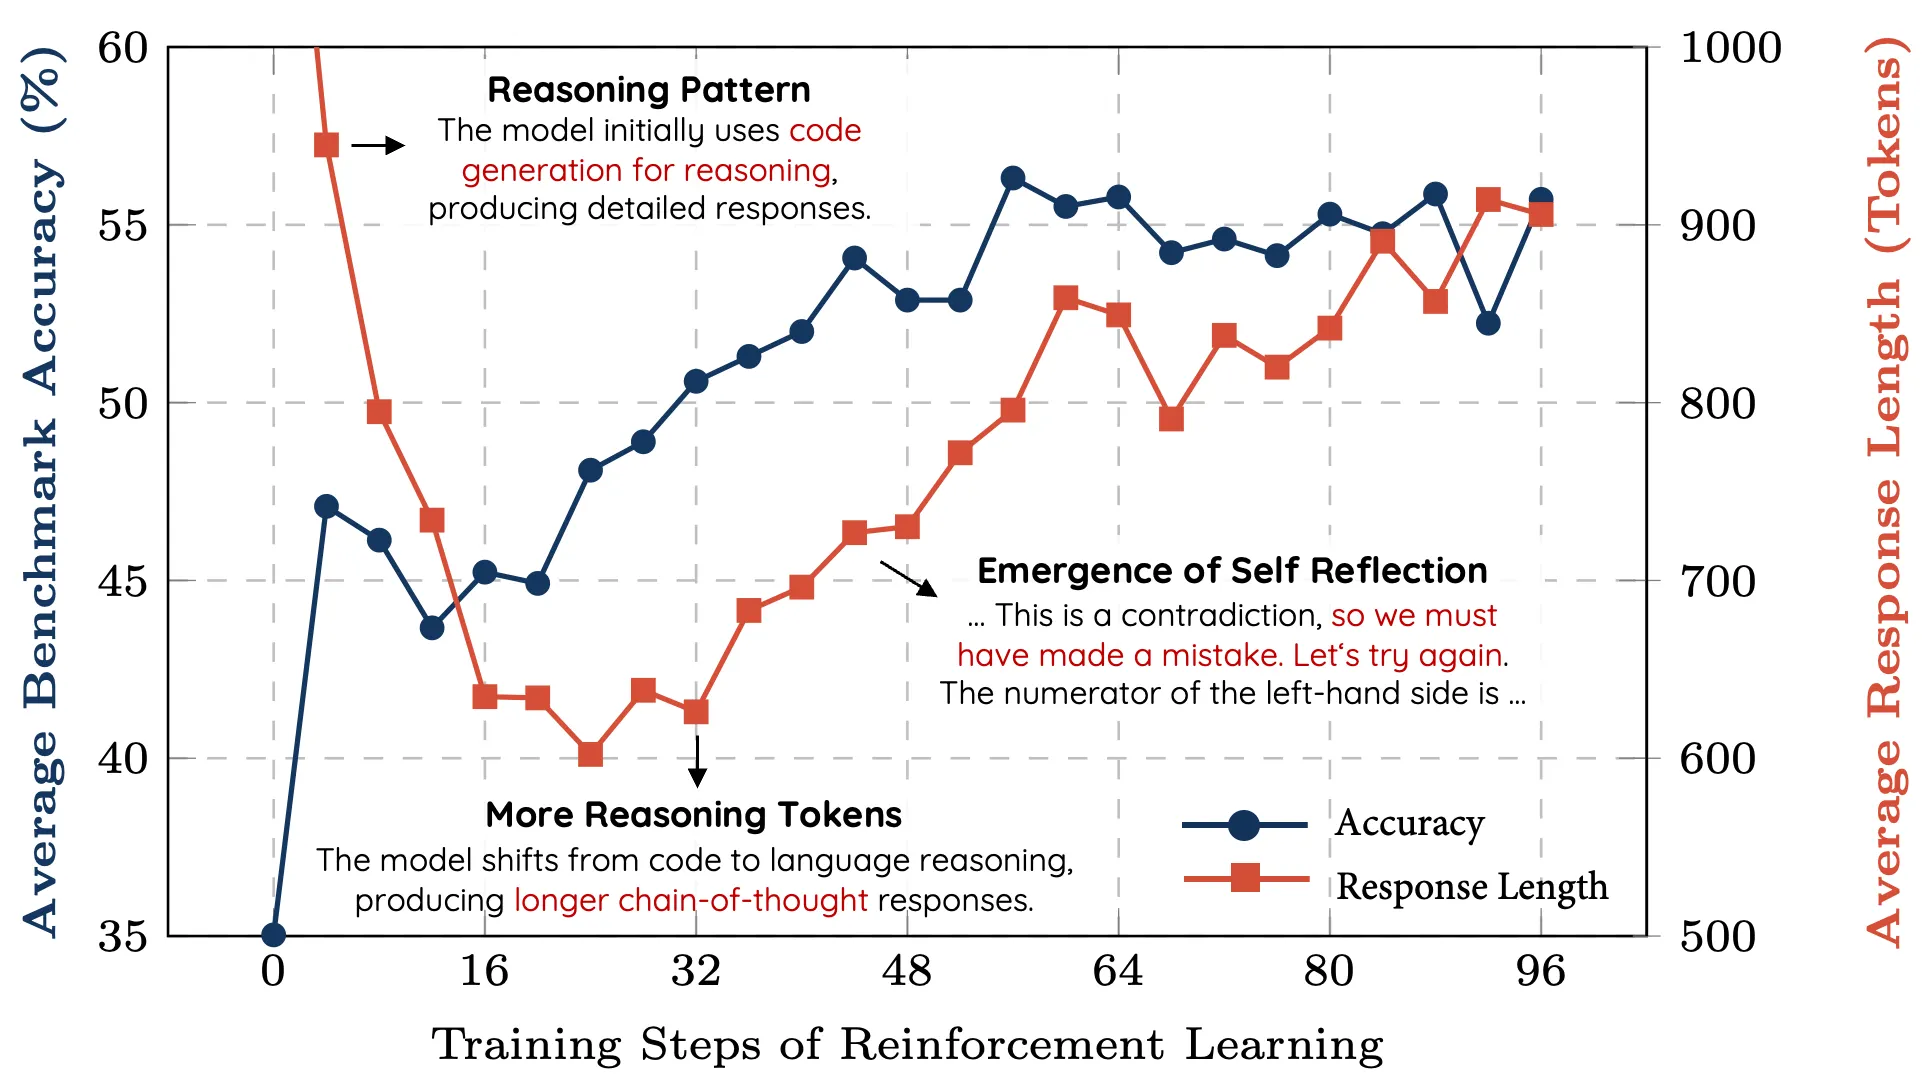
\includegraphics[width=0.92\textwidth]{figs/simplerl_training_curve.png}\\[2pt]
\scriptsize What to expect while GRPO trains: accuracy and response length rise together; self-reflection appears.
\end{column}
\end{columns}
\vspace{4pt}
\begin{tcolorbox}[colback=softgray,colframe=softgray!60!black,boxrule=0.4pt,arc=2pt,left=5pt,right=5pt,top=2pt,bottom=2pt]
\scriptsize
\textbf{DPO:}\; \href{https://colab.research.google.com/drive/1i7aDdW-RHNNPgCCHW9Ky858riqYbrN1R}{\texttt{https://colab.research.google.com/drive/1i7aDdW-RHNNPgCCHW9Ky858riqYbrN1R}}\\
\textbf{GRPO:} \href{https://colab.research.google.com/drive/1hydSFeV8hpTleZTp5EwpoDCjrqRp8JQ7}{\texttt{https://colab.research.google.com/drive/1hydSFeV8hpTleZTp5EwpoDCjrqRp8JQ7}}\\
\textbf{Tip:} Colab Pro is free for students --- \texttt{colab.research.google.com/signup} $\to$ ``No cost for students and educators''.
\end{tcolorbox}
\end{frame}

\begin{frame}[fragile]{The whole of Part 7 in fifteen lines of PyTorch}
\begin{lstlisting}[language=Python,basicstyle=\scriptsize\ttfamily]
def grpo_loss(model, ref_model, batch, eps=0.2, beta=0.04):
    logits     = model(batch["input_ids"]).logits          # current policy
    ref_logits = ref_model(batch["input_ids"]).logits      # frozen reference
    # log-prob of each generated token: the same quantity as in the SFT loss
    logprobs     = token_logprobs(logits,     batch["labels"])
    ref_logprobs = token_logprobs(ref_logits, batch["labels"])
    kl = torch.exp(ref_logprobs - logprobs) - (ref_logprobs - logprobs) - 1
    # group-relative advantages: rewards has shape [num_prompts, G]
    r = batch["rewards"]
    advantages = (r - r.mean(dim=1, keepdim=True)) / (r.std(dim=1, keepdim=True) + 1e-8)
    advantages = advantages.reshape(-1, 1)                  # broadcast to every token
    # PPO-style clipped surrogate + KL penalty
    ratio = torch.exp(logprobs - batch["old_logprobs"])
    surr1 = ratio * advantages
    surr2 = torch.clamp(ratio, 1 - eps, 1 + eps) * advantages
    return -torch.min(surr1, surr2).mean() + beta * kl.mean()
\end{lstlisting}
\vspace{-2pt}
\footnotesize
\begin{itemize}\setlength{\itemsep}{1pt}
  \item \texttt{logprobs}: the same $\log p_\theta(y_t\mid x, y_{<t})$ as in the SFT loss (Part 4). \quad \texttt{advantages}: the worked example of step 2.
  \item \texttt{surr1/surr2}: the PPO clip; \texttt{kl}: the leash (Part 5). Simplified from TRL's \texttt{GRPOTrainer} (which also masks padding, handles several update epochs).
\end{itemize}
\end{frame}
